%!TEX program = xelatex
% 完整编译方法 1 pdflatex -> bibtex -> pdflatex -> pdflatex
% 完整编译方法 2: xelatex -> bibtex -> xelatex -> xelatex
\documentclass[lang=cn,11pt]{elegantpaper}

\title{写他妈的}

% 不需要版本信息, 直接注释即可
% \version{0.07}
% 不需要时间信息的话, 需要把 \today 删除. 
\date{}


% 如果想修改参考文献样式, 请把这行注释掉
% \usepackage[authoryear]{gbt7714}  % 国标

\begin{document}

\section{写在前面}
2019年12月起开始在我国湖北武汉地区流行的新冠肺炎是继2003年后的又一次类SARS病毒带来的灾难, 它的传染力十分强大. 但经过我国政府以及人民不惜代价的努力奋斗, 此次病毒在“人民战争”(引自毛泽东)的汪洋大海之中已经初显颓势. 如\figref{fig:map} , 展示的是我国各省份累计确诊的人数, 颜色越深代表确诊人数越多.
\begin{figure}[htbp]
  \centering
  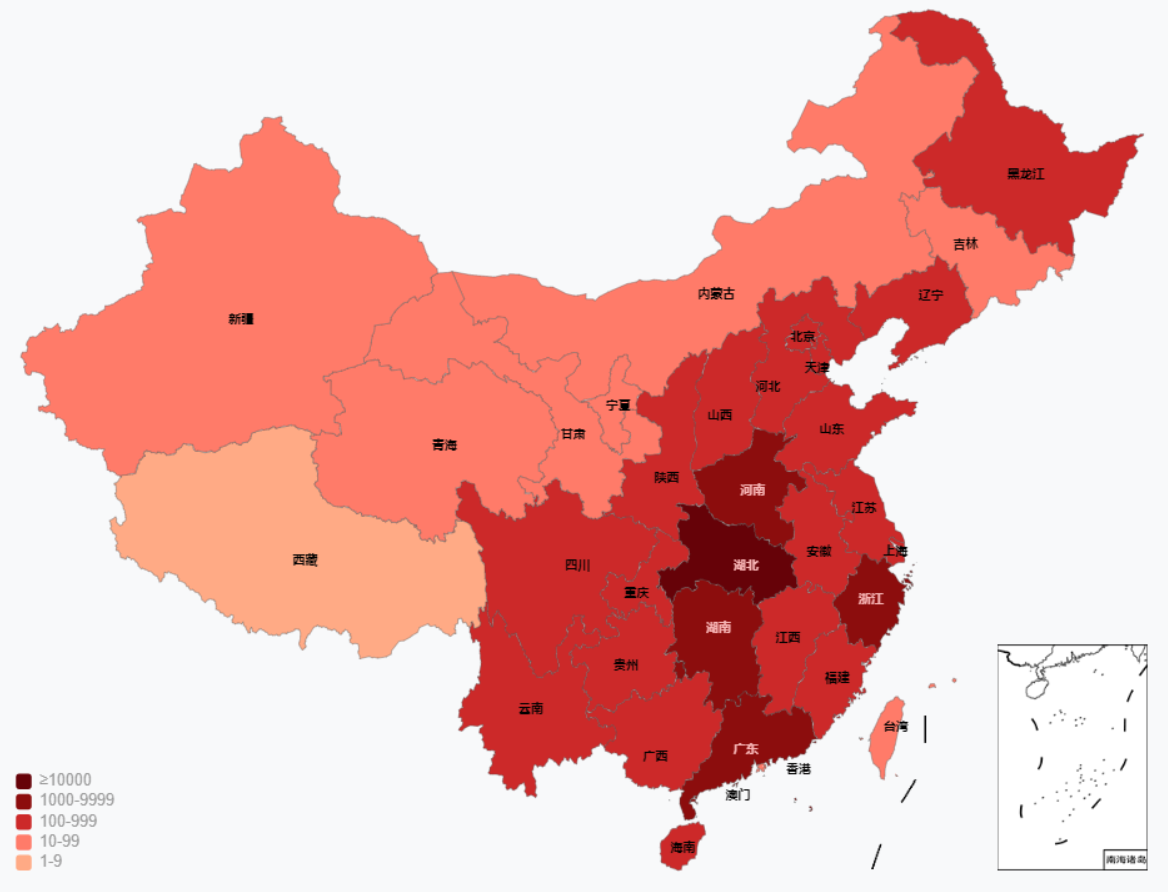
\includegraphics[width=0.6\textwidth]{map}
  \caption{全国疫情地图. \label{fig:map}}
\end{figure}

至少此时此刻(2020.2.29), 我国的情况已经明显好转, 除重灾区湖北以外各地都有组织有序地开始了复工工作的准备. 站在这次灾难即将过去的时刻, 我们试着从各方面的数据之中寻找一些有用的信息, 来为应对下一次类似灾难做好十足的准备. 

\section{问题确定}
对于“对何种问题进行研究”这一问题, 我们有了很多想法. 首先列出我们所能收集到的数据集: 
\begin{center}
  \begin{itemize}
    \item 谣言数据;
    \item 2019-nCov病毒序列等.
    \item 肺炎患者肺部CT扫描数据;
    \item 人民日报有关疫情微博评论数据;
    \item 关于各城市、国家的确诊、疑似、死亡等数据的时间序列; 
  \end{itemize}
\end{center}
在这些数据集的基础上, 我们考虑了以下问题:
\subsubsection*{对于疫情期间的谣言进行甄别.} 
\begin{figure}[htbp]
  \centering
  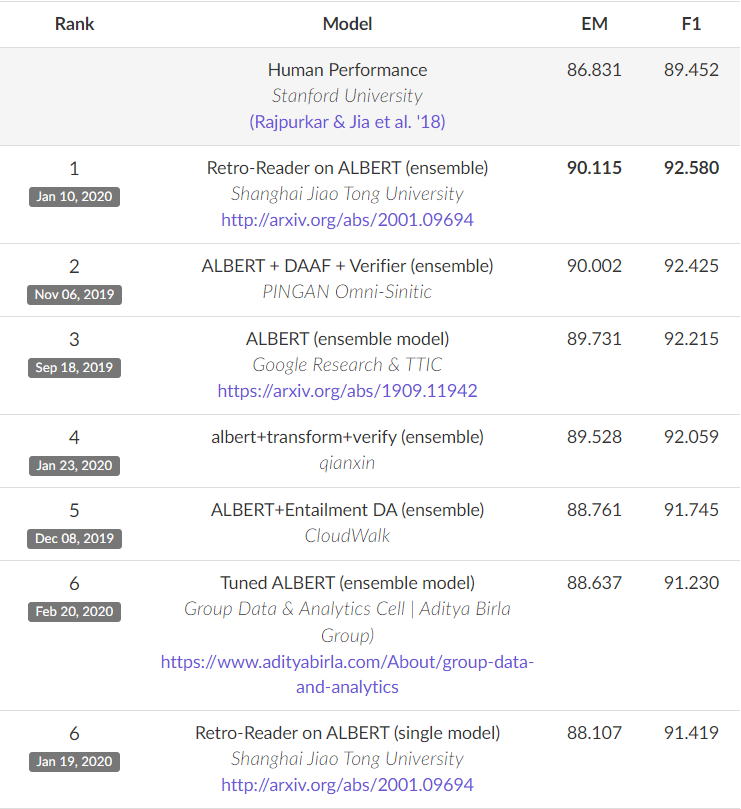
\includegraphics[width=0.55\textwidth]{rank}
  \caption{语言理解模型排名. \label{fig:rank}}
\end{figure}
对于此问题的解决想法是基于Google开发的BERT模型(引)对于谣言文本进行分析, 并且使用机器学习找出谣言具有的普遍特征, 从而对于网络上普遍流传的言论是否是谣言进行判断. 由于BERT模型是开源的, 并且Google也已经使用强大的算力对其进行了长时间的训练, 因此使用者只需要对其进行微调便可以针对特定的问题来应用. 如\figref{fig:rank} 展示的是语言理解模型的排名, 可以看到排名靠前的大多都是基于BERT改进的模型. 但由于时间紧迫, 我们并没有足够的精力来学习此种模型的原理, 因此暂不对此问题做深一步研究. 
\subsubsection*{对于患者肺部CT图进行分析来判断其是否患新型冠状肺炎.}
由于神经网络以及TensorFlow的发明, 对于单一类型的图像进行识别并分类已经不算是一个特别困难的问题. 如神经网络的典型例子, 对于手写数字集(MINST)使用神经网络构建的机器学习模型进行识别, 正确率已经可以达到相当高(引). 但由于可以收集到的肺部CT图数量并不是十分大, 而且位置也不一致, 需要花费大量时间对图像进行剪切. 因此也不对此问题做更进一步的探讨. 
\subsubsection*{使用新冠肺炎病毒的DNA序列对于可能的治疗药物进行预测. }
类似的问题已经有很多研究, 如中国矿业大学陈兴团队对于未知疾病的新型药物进行预测. 可以通过建立病毒相似性网络以及病毒与药物的关联网络以及药物之间的结构相似性及功能相似性网络从而挖掘出可能的起效果的药物. 但同样由于专业知识的缺乏以及时间并不充裕, 这些网络的建立都显得较为困难, 因此不对此问题做深入研究. 
\subsubsection*{对于瘟疫后的经济恢复速度进行预测. }
在大部分企业经过长达一个多月的停工停产后, 经济一定会受到重创, 因此对于经济的恢复做出预测就显得比较重要. 由SARS后的恢复曲线来看, 疫情过后会有小幅度的反弹. 而且第一产业恢复较快, 在疫情刚结束就有明显的反弹, 第二产业次之, 第三产业则恢复速度最慢. 而当今的中国第三产业占比更大, 因此有理由相信这次已经对于经济的影响要远远大于SARS. 由于此类大型灾难次数较少, 因此也没有足够的数据对此类灾后经济恢复模型进行分析, 于是就此作罢. 
\subsubsection*{使用模型预测确诊数量. }
此方法是最基本的, 也是最容易想到的, 并且为了使模型具有解释意义, 一般会使用SIR模型和SEIR模型. 类似的研究在疫情早期便有了结果, 如西安交通大学与加拿大约克大学以及陕西师范大学合作建立的传播动力学模型(引), 但从后续结果来看, 此研究对于疫情发展的估计过于乐观. 使用模型对于确诊人数进行预测是相对容易解决的一类问题. 

在权衡各方面因素后, 我们决定使用SEIR模型通过机器学习的方法对于确诊数量进行预测.
\section{模型建立} 
SEIR模型是较为成熟和常用的流行病预测模型, 所研究的传染病有一定的潜伏期, 与病人接触过的健康人并不马上患病, 而是成为病原体的携带者. 有关SARS的传播动力学研究多数采用的是SIR或SEIR模型. 该模型模拟了传染病的传染途径, 从易感者到潜伏者到感染者再到康复者, 通过各环节的转化率、治愈率等对传染病的传播规模及时间进行预测. 
\subsection{人群划分}
S类, 易感者( Susceptible ), 是指未得病, 但缺乏免疫能力, 与感染者接触后易受到感染;

E类, 潜伏者( Exposed ), 指接触过感染者, 但暂无能力传染给其他人的人, 对潜伏期长的传染病适用;

I类, 感染者( Infective ), 指染上传染病的人, 可以传播给S类成员;

R类, 康复者( Recovered ), 指被隔离或因病愈而具有免疫力的人. 如免疫期有限, R类成员可以重新变成S类.



\subsection{建立方程}
\begin{center}	
    \begin{tabular}{l c}
      \hline
      指标 & 模型参数 \\
      \hline
      $N$&人口总数    \\
      $E$&潜伏者初始值\\
      $I$&感染者初始值\\
      $S$&易感者初始值\\
      $R$& 治愈者初始值 \\
      $r_1$&每个感染者每天有效接触的平均人数\\
      $r_2$&每个潜伏者每天有效接触的平均人数\\
      $\beta_1$&感染者传染正常人的传染概率\\
      $\beta_2$&潜伏者传染正常人的传染概率\\
      $\alpha$&潜伏者转化为感染者概率 \\
      $\gamma$&每天被治愈的病人占总数的比例\\    
      \hline
    \end{tabular}
 \end{center}
 
结合实际情况, 易感人群在一开始会经历潜伏期, 一段时间后才出现症状, 因此假设潜伏者按照概率$\alpha$ 转化为为感染者:
\large
\begin{align*}
S_n&=S_{n-1}-r_1\beta_1 I_{n-1}\frac{S_{n-1}}{N} \\
E_n&=E_{n-1}+r_1\beta_1 I_{n-1}\frac{S_{n-1}}{N} - \alpha E_{n-1} \\ I_n&=I_{n-1}+\alpha E_{n-1}-\gamma I_{n-1}\\
R_n&=R_{n-1}+\gamma I_{n-1}\\
N&=S+E+I+R.
\end{align*}
\normalsize
但通过报导, 此次的新冠肺炎病毒在潜伏期也具有相当高传染性, 因此我们引入$\beta _2$与$r_2$, 潜伏者以$\beta_2$传染概率将健康的易感者转变为潜伏者. 而潜伏者每天接触的健康易感者人数为$r_2$. 因此要在$\frac{dS}{dt}$和$\frac{dE}{dt}$中添加潜伏者的影响项, 修改后的公式如下:
\large
\begin{align*}
\frac{dS}{d t}&=-r_1\beta_1 I\frac{S}{N}-r_2\beta _2E\frac{S}{N} \\
\frac{dE}{d t}&=r_1\beta_1 I\frac{S}{N}+r_2\beta _2E\frac{S}{N}-\alpha E\\
\frac{dI}{d t}&=\alpha E-\gamma I\\
\frac{dR}{d t}&=\gamma I\\
N&=S+E+I+R.
\end{align*}
\normalsize
修改后的迭代方程如下:
\large
\begin{align*}
S_n&=S_{n-1}-r_1\beta_1 I_{n-1}\frac{S_{n-1}}{N}-r_2\beta _2E_{n-1}\frac{S_{n-1}}{N} \\
E_n&=E_{n-1}+r_1\beta_1 I_{n-1}\frac{S_{n-1}}{N}+r_2\beta_2E_{n-1}\frac{S_{n-1}}{N}-\alpha E_{n-1} \\
I_n&=I_{n-1}+\alpha E_{n-1}-\gamma I_{n-1}\\
R_n&=R_{n-1}+\gamma I_{n-1}	\\
N&=S+E+I+R.
\end{align*}
\normalsize


\section{可行性分析}

近年来随着机器学习在各种各样应用领域的成功, 越来越多的领域开始引入机器学习作为工具. 偏微分方程的研究也是其中之一. 偏微分方程判定主要需要解决这样一个问题, 



考虑一个一般的非线性偏微分方程
\large
\begin{equation}
	u_t=\mathcal N(t,x,u_x,u_{xx},...),
\end{equation}
\normalsize
其中$\mathcal N$是一个非线性函数, 角标代表偏微分的方向. 那么我们给定了一系列数据$w_t(x,t)$, 其中$x$为空间中的网格点,$0\leq t\leq M$为时间戳, 我们能否根据空间偏导数的数据来判定这个偏微分方程的形式? 在最近的一些研究中, 有学者采用了神经网络(深度网络)来在这方面有了一些进展.

如果我们能够有一些对于这个方程的先验知识, 比如这个方程大概是一个二次偏微分方程等等, 那么我们便可以通过字典学习的方式来完成这样一个任务.

对于一个具有二次型非线性项的二阶偏微分方程, 我们可以给出它的一般形式.
\large
\begin{equation}
	u_t=\alpha_1+\alpha_2u+\alpha_3u^2+\alpha_4u_x+\alpha_5u_x^2+\alpha_6uu_x+\alpha_7u_{xx}+\alpha_8u_{xx}^2+\alpha_9uu_{xx}+\alpha_{10}u_xu_{xx}
\end{equation}
\normalsize
那么这样的方程的阶数的确定可以根据经验及其物理意义或者是通过数值方法. 那么上面的方程还可以写成
\large
\begin{equation}
	u_t=[1\quad u\quad u^2\quad u_x\quad u_x^2\quad uu_x\quad u_{xx}\quad u_{xx}^2\quad uu_{xx}\quad u_xu_{xx}] \mathbf \alpha
\end{equation}
\normalsize
其中我们可以把它归结为一项是字典项$F_u(t)$, 一项是系数项$\alpha$. 那么这个时候我们可以通过去优化
\large
\begin{equation}
	\min_\alpha \dfrac{1}{2}\sum_{k=1}^M ||u_t(t_k)-F_U(t_k)\alpha||_2^2+\lambda||\alpha||_1
\end{equation}
\normalsize
来获得这样的向量$\alpha$, 从而对于由字典里的函数通过线性组合能够表达出来的函数获得较好的结果. 其中$L_1$正则项的假设是比较自然的, $L_1$范数惩罚往往能够使得向量的坐标趋于稀疏, 因为其导数的线性性质. 在方程阶数增加时, 字典的大小是指数级增长的, 不过偏微分方程一般无法张满整个字典, 往往都是其中的几项起着作用. 所以稀疏的表示往往更符合这样具有物理含义的偏微分方程的规律, 这也符合奥卡姆的剃刀原理.

另外一种思路便是不加上这样偏微分方程非线项是二次型的假设, 直接使用神经网络来去近似这样的非线性性, 也就是说我们需要习得一个网络$\mathcal N$使得$u_t=\mathcal N(u,u_x,u_{xx})$(更高阶的字典也可以实现). 通过选择激活函数跟调整网络超参数来得到一个比较好的近似. 我们的方法的灵感也是来源于这里. 虽不过这种方法在失去了假设的情况下缺少可解释性. 我们并不知道这样的神经网络到底能不能或者在什么程度上表示什么形式的多么复杂的偏微分方程. 并且这样用神经网络复原出来的方程在长时间的演变中能否真的近似原方程. 不过SEIR是多元常微分方程, 通过变量替换得出的偏微分表达式其实是类似于$\dfrac{1}{u}$型的. 所以其实究竟这样的神经网络能否真的近似SEIR模型的差分, 我们并不完全确定. 并且这样的方法在理想的条件下的偏微分方程恢复中, 已经显现出了对噪声的敏感性(主要是加上了噪声后, 数值上对偏导数的近似计算的误差会累积, 并且网格越密这样的误差就会越大). 我们面临的情况甚至更加复杂, 数据更杂乱更少, 噪声复杂, 并且可能训练样本的分布情况并不一定相同, 不过我们还是决定试一试.


\section{模型实践}

我们采用了一个双层全联接的神经网络$\mathcal N$, 构建了字典$[S(t),E(t),I(t),R(t),S(t)S(t),...,R(t)R(t)]$, 即所有的二次项, 希望能够通过第$t$时刻的任何一个城市的$S,E,I,R$的值, 通过神经网络来预测这个城市$E,I$在$t$时刻向前的差分. 

因为我们的数据与原复原偏微分方程的数据量上差了不止一个数量级, 并且我们也并不知道SEIR模型中的各个量在$t$时刻的值, 于是我们作出以下假设, 
\begin{enumerate}
	\item 以天为最小时间长度, 虽然数据源是以小时为单位统计的, 但是我们认为统计数据的结果收到太多因素的影响, 这样的统计方式缺乏稳定性, 相当于反而增大了噪声与蕴含有效信息之间的比例.
	\item 合并E与I项, 计作E. 对任何一个城市以四天后的确诊人数减去今天的确诊人数作为目前在城市里游荡的有感染能力的潜在感染者.
	\item 将潜在感染人数设为密切接触人数, 并且对密切接触人数确诊人数作出线性假设, 以估计各个城市各个时间的潜在感染人数, 依照2月28日公布的658587为基准成比例计算出所有城市$t$时刻的潜在感染人数, 对于一个城市再由这个感染人数按比例推算出$t$时刻之前的所有感染人数. 
\end{enumerate}

将所有城市的随机分为80\%训练数据与20\%测试数据, 每一个样本包括这个城市在66天(t时刻)的$E(t)$的差分$\Delta E_{city}(t)$与其对应的$S,E,R$的值. 再在训练数据中的按城市分出10\%的验证数据. 性能度量设为Absolute mean error(因为我们还是觉得这样的表示应该是相对稀疏的), 优化算法设为随机梯度下降, 学习率0.03, 每层网络十个tanh单元, 一共两层全连接, 最后一个输出单元.

\begin{equation}
	\min_{\mathcal N} \dfrac{1}{232*66}\Delta \sum_{\text{all 232 cities, 66 days}}\Big|E_{city}(t)-\mathcal N(S_{city}(t),E_{city}(t),R_{city}(t))\Big|
\end{equation}



\newpage
\nocite{*}

% 如果想修改参考文献样式(非国标), 请把下行取消注释, 并换成合适的样式(比如 unsrt, plain 样式). 
\bibliographystyle{unsrt}
\bibliography{wpref}

\end{document}
